To stop the weak radiation we use the so-called passive veto, which consists of a lead shielding inside which we will place the TRITIUM detector. This lead shielding is used to stop external particles before they reach the tritium detector, affecting the tritium measurement. It will work for particle energies below $200~\MeV/$nucleon, which is mainly the earth's natural radioactivity and the weak component of cosmic radiation.

This lead shielding consists of $158$ lead bricks with ultra-low instrinsec radioactivity, whose thickness are $25~\mm$. .They are shaped like a shevron, shown in the figure \ref{subfig:LeadBricks}, specially designed for a perfect fit and easy assembly. As can be seen in the figures \ref{subfig:TwoLayers} and \ref{subfig:TwoLayers2}, these lead bricks are arranged in two layers leaving a total thickness of the lead shielding walls of $50~\mm$ and the space between the lead bricks in the inner layer is overlaid with a lead brick of the outer layer to avoid possible entry of radiation.

\begin{figure}[htbp]
 \centering
  \subfloat[Lead bricks.]{
   \label{subfig:LeadBricks}
    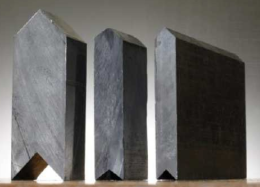
\includegraphics[width=0.3\textwidth]{3DesignPrinciples/34BackgroundRejectionSystem/LeadBricks.png}}
  \subfloat[Two layers for the lead bricks of the shielding.]{
   \label{subfig:TwoLayers}
    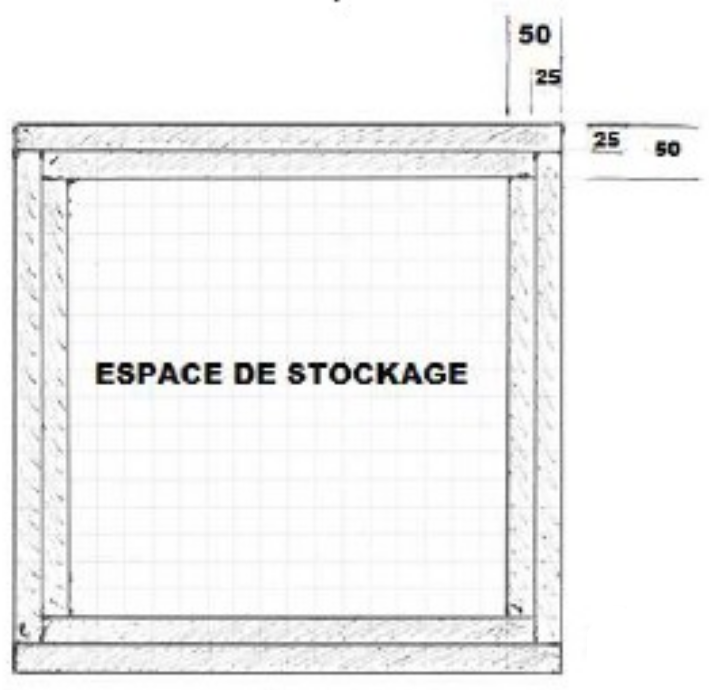
\includegraphics[width=0.3\textwidth]{3DesignPrinciples/34BackgroundRejectionSystem/TwoLayers.png}}
   %\newline
  \subfloat[Two layers for the lead bricks of the shielding.]{
   \label{subfig:TwoLayers2}
    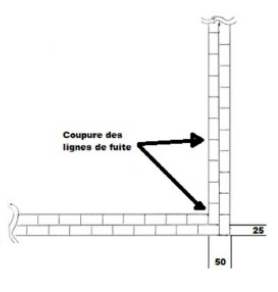
\includegraphics[width=0.3\textwidth]{3DesignPrinciples/34BackgroundRejectionSystem/TwoLayers2.png}}
 \caption{Lead Bricks and their arrangement in the lead shielding.}
 \label{fig:LeadBricksAndArrangement}
\end{figure}

Mechanical engineering department of CENBG has designed a special aluminum structure, shown in figure \ref{fig:AluminiumStructure}, to support the total weight of the lead bricks, $2.4$ tons.

\begin{figure}[htbp]
 \centering
  \subfloat[Aluminium structure scheme.]{
   \label{subfig:AluminiumStructureScheme}
    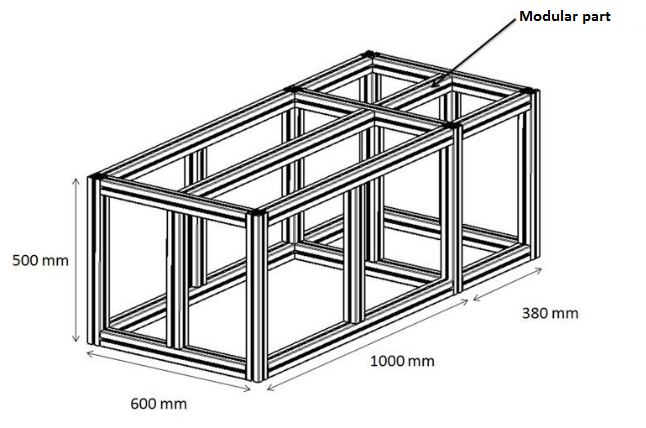
\includegraphics[width=0.45\textwidth]{3DesignPrinciples/34BackgroundRejectionSystem/AluminiumStructureScheme.png}}
  \subfloat[Aluminium structure of TRITIUM monitor.]{
   \label{subfig:AluminiumStructure}
    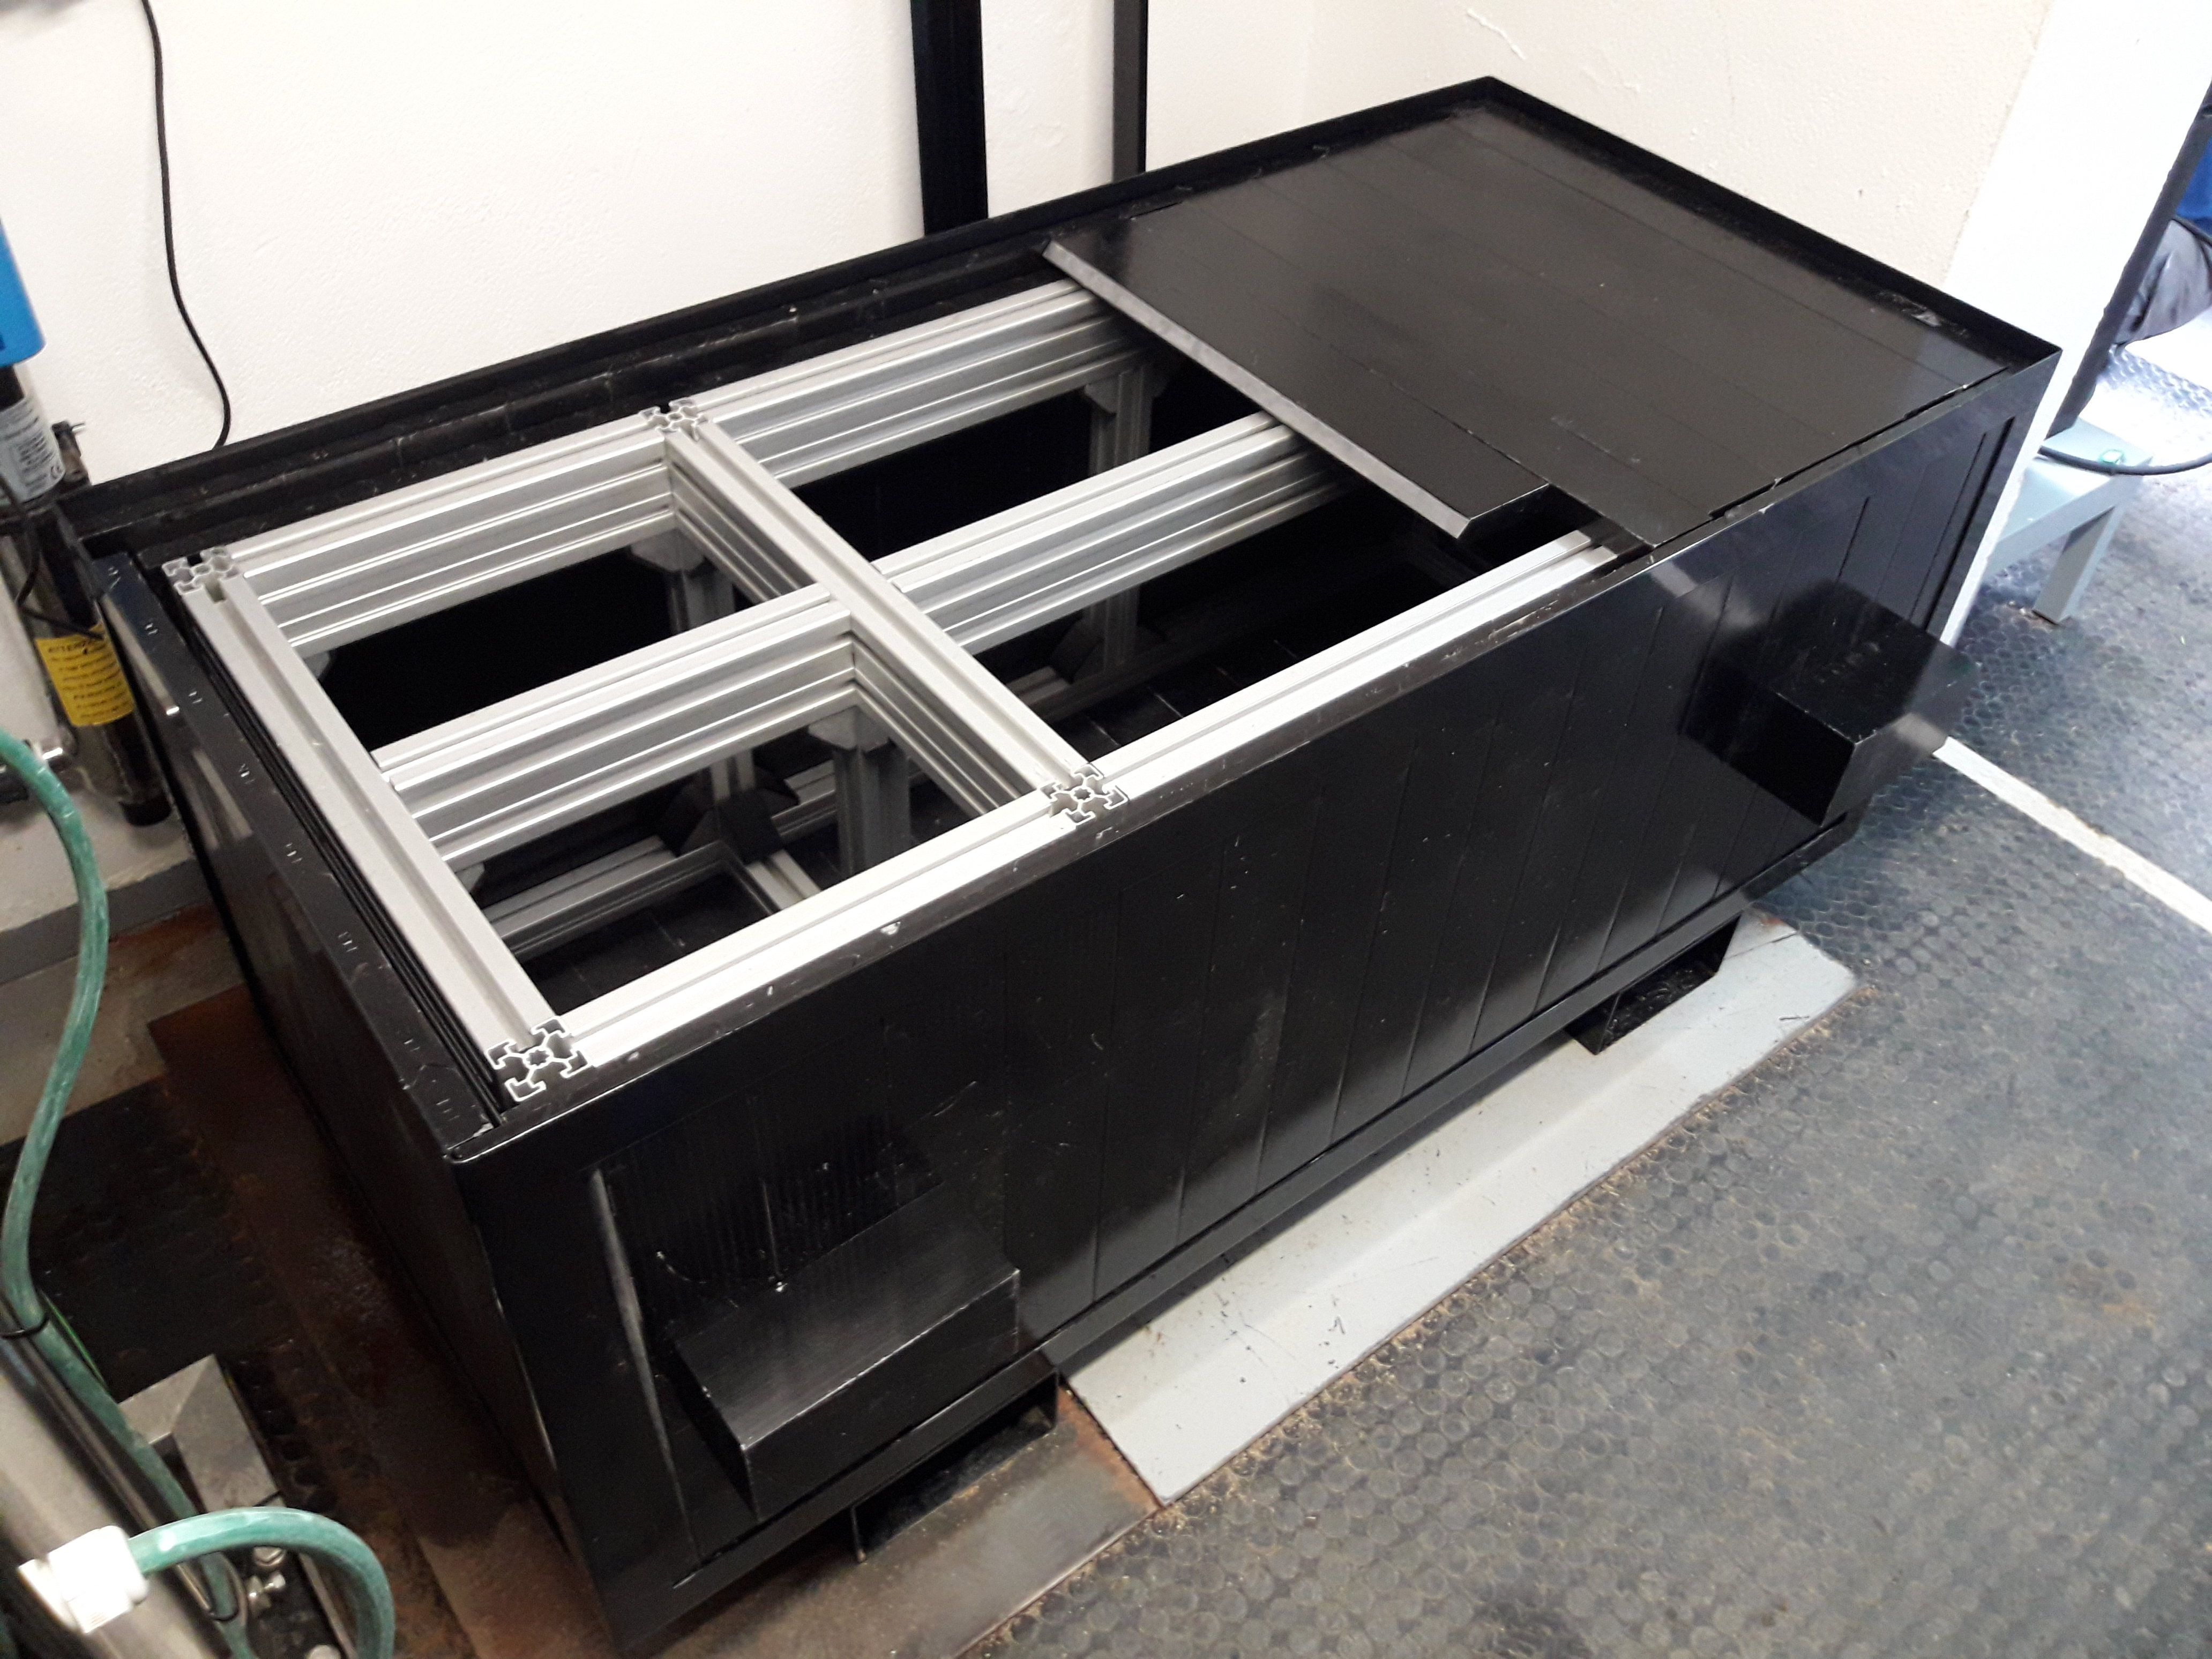
\includegraphics[width=0.4\textwidth]{3DesignPrinciples/34BackgroundRejectionSystem/AluminiumStructure.jpg}}
    \caption{Lead Bricks and their arrangement in the lead shielding.}
 \label{fig:AluminiumStructure}
\end{figure}

The internal space of this lead shielding is arranged in two parts, shown in figure \ref{fig:LeadBricksAndArrangement}. The one, larger, has an internal dimensions of $90.5~\cm$ long, $41~\cm$ deep, and $51~\cm$ high and it will be used to place the TRITIUM detector. The other, smaller, has an internal dimensions of $33~\cm$ long, $41~\cm$ deep, and $51~\cm$ high and it will serve to place the electronic system necessary to collect and store data. The external dimensions of this lead shielding are $148~\cm$ long, $60~\cm$ deep and $70~\cm$ high and a weight of $2.5$ tons.

